\documentclass[conference]{IEEEtran}

% correct bad hyphenation here
\hyphenation{op-tical net-works semi-conduc-tor}
\usepackage{amsmath}
\usepackage{comment}
\usepackage{graphicx}
%\usepackage{cases}
%\usepackage{subeqnarray}

\begin{document}
%
% paper title
% Titles are generally capitalized except for words such as a, an, and, as,
% at, but, by, for, in, nor, of, on, or, the, to and up, which are usually
% not capitalized unless they are the first or last word of the title.
% Linebreaks \\ can be used within to get better formatting as desired.
% Do not put math or special symbols in the title.
\title{Multiple Object Tracking with DeepSORT, LSTM, and More Kalman Filters}
%
%
% author names and IEEE memberships
% note positions of commas and nonbreaking spaces ( ~ ) LaTeX will not break
% a structure at a ~ so this keeps an author's name from being broken across
% two lines.
% use \thanks{} to gain access to the first footnote area
% a separate \thanks must be used for each paragraph as LaTeX2e's \thanks
% was not built to handle multiple paragraphs
%

\author{
    Shangning Xu,
    Zhongye Wang,
    Xinyu Zhan
}

% The paper headers
% \markboth{Journal of \LaTeX\ Class Files,~Vol.~13, No.~9, September~2014}%
% {Shell \MakeLowercase{\textit{et al.}}: Bare Demo of IEEEtran.cls for Journals}
% The only time the second header will appear is for the odd numbered pages
% after the title page when using the twoside option.
%
% *** Note that you probably will NOT want to include the author's ***
% *** name in the headers of peer review papers.                   ***
% You can use \ifCLASSOPTIONpeerreview for conditional compilation here if
% you desire.


% make the title area
\maketitle

% As a general rule, do not put math, special symbols or citations
% in the abstract or keywords.
\begin{abstract}
The abstract goes here.
\end{abstract}

% Note that keywords are not normally used for peerreview papers.
\begin{IEEEkeywords}
IEEEtran, journal, \LaTeX, paper, template.
\end{IEEEkeywords}


\IEEEpeerreviewmaketitle



\section{Introduction}

\IEEEPARstart{T}{his}

\section{Understanding and Re-implementing DeepSort}

\section{Using LSTM for MOT}

\section{Using More Kalman Filters}

\subsection{Extended State Space}

Extending the state vector is a natural idea. A state space of higher dimensions should be able to characterize the state of object in video with more precision. The constant velocity model proposed by \cite{Wojke2017simple}, where the position, aspect ratio and height of a track changes linearly over time, is simple and should apply to most pedestrians, but fail to account for some complex cases, such as the one shown in Fig.~\ref{fig:example-of-nonlinearity}. Therefore, we augment the state space first with acceleration (2nd order) using the constant acceleration model and later higher order terms.

\begin{figure}[t]
    \centering
    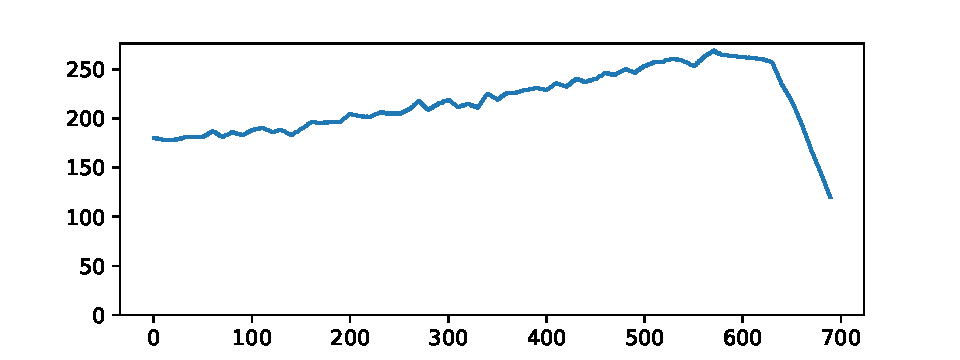
\includegraphics[width=\linewidth]{fig/accelerating-pedestrian-height-plot.pdf}
    \caption{An example of the nonlinear behavior of a state variable. The height of the pedestrian 70 in the sequence MOT16-02 is plotted against time. The pedestrian first moves towards camera and then exits the field of view.}
    \label{fig:example-of-nonlinearity}
\end{figure}

We give an example of augmenting the state space with acceleration below. The new state vector is
\[
    s = [x, y, a, h, v_x, v_y, v_a, v_h, a_x, a_y, a_a, a_h].
\]

Using the example of $x$-coordinate, the state-transition equation is
\[
    x_{k + 1} = x_k + v_{xk} \Delta t + \frac{1}{2} a_{xk} \Delta t^2.
\]

For the velocity, the equation is
\[
    v_{x, k + 1} = v_{xk} + a_{xk} \Delta t.
\]

The equations for other state variables are similar. The state-transition equation for the state vector is
\[
    s_{k + 1} = Fs_k + w_k,
\]
where $F$ is the new state-transition matrix
\[
    F = \begin{bmatrix}
        I_4 & \Delta t I_4 & \frac{1}{2} \Delta t^2 I_4\\
        \mathcal{O} & I_4 & \Delta t I_4\\
        \mathcal{O} & \mathcal{O} & I_4
    \end{bmatrix}
\]
and $w_k$ is noise.

The measurement matrix is
\[
    H = [I_4, \mathcal{O}, \mathcal{O}].
\]

In a similar fashion, the state vector with constant $k$-order terms is a $4k$-dimensional vector. The state-transition matrix is $4k \times 4k$ and the measurement matrix $4 \times 4k$ in this case.

\subsection{Filtering on Features}

\section{Conclusion}

\bibliographystyle{IEEEtran}
\bibliography{Ref}

\end{document}
